\documentclass{ximera}
\graphicspath{  %% When looking for images,
{./}            %% look here first,
{./pictures/}   %% then look for a pictures folder,
{../pictures/}  %% which may be a directory up.
{../../pictures/}  %% which may be a directory up.
{../../../pictures/}  %% which may be a directory up.
{../../../../pictures/}  %% which may be a directory up.
}

\usepackage{listings}
\usepackage{circuitikz}
\usepackage{xcolor}
\usepackage{amsmath,amsthm}
\usepackage{subcaption}
\usepackage{graphicx}
\usepackage{tikz}
\usepackage{tikz-3dplot}
\usepackage{amsfonts}
\usepackage{mdframed} % For framing content
\usepackage{tikz-cd}

  \renewcommand{\vector}[1]{\left\langle #1\right\rangle}
  \newcommand{\arrowvec}[1]{{\overset{\rightharpoonup}{#1}}}
  \newcommand{\ro}{\texttt{R}}%% row operation
  \newcommand{\dotp}{\bullet}%% dot product
  \renewcommand{\l}{\ell}
  \let\defaultAnswerFormat\answerFormatBoxed
  \usetikzlibrary{calc,bending}
  \tikzset{>=stealth}
  




%make a maroon color
\definecolor{maroon}{RGB}{128,0,0}
%make a dark blue color
\definecolor{darkblue}{RGB}{0,0,139}
%define the color fourier0 to be the maroon color
\definecolor{fourier0}{RGB}{128,0,0}
%define the color fourier1 to be the dark blue color
\definecolor{fourier1}{RGB}{0,0,139}
%define the color fourier 1t to be the light blue color
\definecolor{fourier1t}{RGB}{173,216,230}
%define the color fourier2 to be the dark green color
\definecolor{fourier2}{RGB}{0,100,0}
%define teh color fourier2t to be the light green color
\definecolor{fourier2t}{RGB}{144,238,144}
%define the color fourier3 to be the dark purple color
\definecolor{fourier3}{RGB}{128,0,128}
%define the color fourier3t to be the light purple color
\definecolor{fourier3t}{RGB}{221,160,221}
%define the color fourier0t to be the red color
\definecolor{fourier0t}{RGB}{255,0,0}
%define the color fourier4 to be the orange color
\definecolor{fourier4}{RGB}{255,165,0}
%define the color fourier4t to be the darker orange color
\definecolor{fourier4t}{RGB}{255,215,0}
%define the color fourier5 to be the yellow color
\definecolor{fourier5}{RGB}{255,255,0}
%define the color fourier5t to be the darker yellow color
\definecolor{fourier5t}{RGB}{255,255,100}
%define the color fourier6 to be the green color
\definecolor{fourier6}{RGB}{0,128,0}
%define the color fourier6t to be the darker green color
\definecolor{fourier6t}{RGB}{0,255,0}

%New commands for this doc for errors in copying
\newcommand{\eigenvar}{\lambda}
%\newcommand{\vect}[1]{\mathbf{#1}}
\renewcommand{\th}{^{\text{th}}}
\newcommand{\st}{^{\text{st}}}
\newcommand{\nd}{^{\text{nd}}}
\newcommand{\rd}{^{\text{rd}}}
\newcommand{\paren}[1]{\left(#1\right)}
\newcommand{\abs}[1]{\left|#1\right|}
\newcommand{\R}{\mathbb{R}}
\newcommand{\C}{\mathbb{C}}
\newcommand{\Hilb}{\mathbb{H}}
\newcommand{\qq}[1]{\text{#1}}
\newcommand{\Z}{\mathbb{Z}}
\newcommand{\N}{\mathbb{N}}
\newcommand{\q}[1]{\text{``#1''}}
%\newcommand{\mat}[1]{\begin{bmatrix}#1\end{bmatrix}}
\newcommand{\rref}{\text{reduced row echelon form}}
\newcommand{\ef}{\text{echelon form}}
\newcommand{\ohm}{\Omega}
\newcommand{\volt}{\text{V}}
\newcommand{\amp}{\text{A}}
\newcommand{\Seq}{\textbf{Seq}}
\newcommand{\Poly}{\textbf{P}}
\renewcommand{\quad}{\text{    }}
\newcommand{\roweq}{\simeq}
\newcommand{\rowop}{\simeq}
\newcommand{\rowswap}{\leftrightarrow}
\newcommand{\Mat}{\textbf{M}}
\newcommand{\Func}{\textbf{Func}}
\newcommand{\Hw}{\textbf{Hamming weight}}
\newcommand{\Hd}{\textbf{Hamming distance}}
\newcommand{\rank}{\text{rank}}
\newcommand{\longvect}[1]{\overrightarrow{#1}}
% Define the circled command
\newcommand{\circled}[1]{%
  \tikz[baseline=(char.base)]{
    \node[shape=circle,draw,inner sep=2pt,red,fill=red!20,text=black] (char) {#1};}%
}

% Define custom command \strikeh that just puts red text on the 2nd argument
\newcommand{\strikeh}[2]{\textcolor{red}{#2}}

% Define custom command \strikev that just puts red text on the 2nd argument
\newcommand{\strikev}[2]{\textcolor{red}{#2}}

%more new commands for this doc for errors in copying
\newcommand{\SI}{\text{SI}}
\newcommand{\kg}{\text{kg}}
\newcommand{\m}{\text{m}}
\newcommand{\s}{\text{s}}
\newcommand{\norm}[1]{\left\|#1\right\|}
\newcommand{\col}{\text{col}}
\newcommand{\sspan}{\text{span}}
\newcommand{\proj}{\text{proj}}
\newcommand{\set}[1]{\left\{#1\right\}}
\newcommand{\degC}{^\circ\text{C}}
\newcommand{\centroid}[1]{\overline{#1}}
\newcommand{\dotprod}{\boldsymbol{\cdot}}
%\newcommand{\coord}[1]{\begin{bmatrix}#1\end{bmatrix}}
\newcommand{\iprod}[1]{\langle #1 \rangle}
\newcommand{\adjoint}{^{*}}
\newcommand{\conjugate}[1]{\overline{#1}}
\newcommand{\eigenvarA}{\lambda}
\newcommand{\eigenvarB}{\mu}
\newcommand{\orth}{\perp}
\newcommand{\bigbracket}[1]{\left[#1\right]}
\newcommand{\textiff}{\text{ if and only if }}
\newcommand{\adj}{\text{adj}}
\newcommand{\ijth}{\emph{ij}^\text{th}}
\newcommand{\minor}[2]{M_{#2}}
\newcommand{\cofactor}{\text{C}}
\newcommand{\shift}{\textbf{shift}}
\newcommand{\startmat}[1]{
  \left[\begin{array}{#1}
}
\newcommand{\stopmat}{\end{array}\right]}
%a command to give a name to explorations and hints and theorems
\newcommand{\name}[1]{\begin{centering}\textbf{#1}\end{centering}}
\newcommand{\vect}[1]{\vec{#1}}
\newcommand{\dfn}[1]{\textbf{#1}}
\newcommand{\transpose}{\mathsf{T}}
\newcommand{\mtlb}[2][black]{\texttt{\textcolor{#1}{#2}}}
\newcommand{\RR}{\mathbb{R}} % Real numbers
\newcommand{\id}{\text{id}}

\author{Zack Reed} %borrowed from Bart and PEter Selinger
\title{Learning Activity: Matrices are Everywhere!}
\begin{document}
\begin{abstract}
Here we introduce matrices similar to vectors
\end{abstract}
\maketitle


\section{Matrices store and transform data}

Keeping with the convention that \emph{vectors} are arrays of numbers that represent data, we often want to consider not just individual vectors at one time, but collections of vectors. \emph{matrices} allow us to methodologically store and manipulate data vectors.

We'll start with some intuition and basics for now, and then next chapter we'll go into much greater detail about the geometric connections between matrices and vectors.

First, a very basic definition or two:


\begin{definition}

A \emph{matrix} is just a big rectangular array of numbers
\[
M =
\underset{\displaystyle\boldsymbol{5}~\textbf{columns}}{\begin{pmatrix}
  a_{1,1} & a_{1,2} & a_{1,3} & a_{1,4} & a_{1,5} \\
  a_{2,1} & a_{2,2} & a_{2,3} & a_{2,4} & a_{2,5} \\
  a_{3,1} & a_{3,2} & a_{3,3} & a_{1,4} & a_{3,5} \\
  a_{4,1} & a_{4,2} & a_{4,3} & a_{4,4} & a_{4,5}
\end{pmatrix}}
\boldsymbol{4}~\textbf {rows}
\]

We give the \emph{dimensions of a matrix} by stating its number of rows
and columns. Rows come first and columns come second, so $M$ above is
a $(4\times 5)$-matrix. We can use similar notation to talk about
specific entries of a matrix. Above, $a_{i,j}$ is the
$\boldsymbol{(i,j)}${\bf-}\emph{entry} of the matrix $M$. Sometimes,
people write $M_{i,j}$ to mean the $(i,j)$-entry of the matrix $M$.

\end{definition}

For instance, the following is a $4\times 5$ matrix:

\[
M =
\underset{\displaystyle\boldsymbol{5}\textbf{columns}}{
\begin{pmatrix}
4.56 & -2.32 & 3.12 & 0.78 & 1.92 \\
7.13 & 1.25 & -0.67 & 2.89 & -1.05 \\
3.45 & 8.62 & 0.34 & 6.78 & -9.12 \\
2.98 & -5.44 & 3.91 & 4.23 & 0.15
\end{pmatrix}}
\boldsymbol{4}\textbf{rows}
\]

\begin{definition}

    We might also say that a matrix is an \emph{array of vectors}. 
    
    That is, we can think of vectors as either being the rows or columns of a matrix, and thus the matrix is an array of these vectors.

\end{definition}

Because of this, we might at times specify vectors in reference to their position in a matrix, by identifying whether we care to think of the rows as vectors, or the columns as vectors, or both. This often gives the matrix some interpretability.

\begin{example}

    If we consider the columns of $M$ as vectors, we might write the columns of matrix $M$ as: 

    \[
v_1 = \begin{pmatrix} 4.56 \\ 7.13 \\ 3.45 \\ 2.98 \end{pmatrix}, \quad
v_2 = \begin{pmatrix} -2.32 \\ 1.25 \\ 8.62 \\ -5.44 \end{pmatrix}, \quad
v_3 = \begin{pmatrix} 3.12 \\ -0.67 \\ 0.34 \\ 3.91 \end{pmatrix}, \quad
v_4 = \begin{pmatrix} 0.78 \\ 2.89 \\ 6.78 \\ 4.23 \end{pmatrix}, \quad
v_5 = \begin{pmatrix} 1.92 \\ -1.05 \\ -9.12 \\ 0.15 \end{pmatrix}
\]

where the matrix is the array of vectors

    \[
M =
\left[\begin{array}{ccccc}
  v_1 & v_2 & v_3 & v_4 & v_5
\end{array}
\right]
\].

Alternatively, if we take the rows of the matrix, we can write $M$ as:

\[
M =
\left[\begin{array}{c}
  r_1 \\
  r_2 \\
  r_3 \\
  r_4
\end{array}
\right]
\]

where

\[
r_1 = \begin{pmatrix} 4.56 & -2.32 & 3.12 & 0.78 & 1.92 \end{pmatrix}, \quad
r_2 = \begin{pmatrix} 7.13 & 1.25 & -0.67 & 2.89 & -1.05 \end{pmatrix}, \quad \]
\[
r_3 = \begin{pmatrix} 3.45 & 8.62 & 0.34 & 6.78 & -9.12 \end{pmatrix}, \quad
r_4 = \begin{pmatrix} 2.98 & -5.44 & 3.91 & 4.23 & 0.15 \end{pmatrix}
\]\


\end{example}

Either way, the matrix $M$ has $4$ rows and $5$ columns, and so we say that $M$ is a $(4\times 5)$-matrix.


\begin{exploration}\name{Matrix and Vector Connections}

    The distinction between matrices storing rows of vectors and columns of vectors motivates the following, at first simple, characterizations:

    \begin{description}
        \item[As a row vector] A row vector is a vector whose entries have been specifically arranged in row format.
        
        Suppose a bookstore sells a variety of books in a month, say
          $141$ Science Fiction,
          $304$ Fantasy,
          $249$ Mystery,
          $199$ Romance,
          $251$ Historical.
          We can express this data as a row vector:
          \[
          \vec{s} = \begin{pmatrix}141 & 304 & 249 & 199 & 251 \end{pmatrix}
          \]
        \item[As a column vector] A column vector is just like a row vector,
          except is it written vertically:
          \[
          \vec{w}_{\texttt{TR}} = \begin{pmatrix}
            0.5\\ 4 \\ 0 \\ 1\end{pmatrix}
            \qquad
            \begin{array}{l}
            \text{Emails}\\
            \text{Classes}\\
            \text{Projects}\\
            \text{Exercising}
          \end{array}
          \]
          Above, we could suppose that $\vec{w}_{\texttt{TR}}$ represents the
          fact that on Tuesdays and Thursdays, someone spends $0.5$ hours on
          emails, $4$ hours in class, $0$ hours on projects, and $1$ hour
          exercising.
        \end{description}
        
        
        Of course, since mathematics is a human endeavor you will find variations on the notation above, as a common example, some folks use different brackets like these
        \[
        \langle a, b, c\rangle \qquad\text{or}\qquad
        \begin{bmatrix}
          a\\
          b\\
          c
        \end{bmatrix}
        \]
        for an ordered-tuple vectors and column vectors. Ordered tuples and
        row vectors are more convient to write in a line, because they are
        horizontal. On the other hand, column vectors take up less horizontal
        space, and are more convenient when you have vectors with many entries.
        
        
        \begin{definition}
          To switch a row vector into a column vector and vice versa, we use what is called the \emph{transpose} operation:
          \[
          \begin{pmatrix} 1 &  2 & 3 \end{pmatrix}^\transpose =
          \begin{pmatrix} 1 \\ 2 \\ 3 \end{pmatrix}
          \quad\text{and}\quad
          \begin{pmatrix} 1 \\ 2 \\ 3 \end{pmatrix}^\transpose =
          \begin{pmatrix} 1 &  2 & 3 \end{pmatrix}
          \]
        \end{definition}

        At times it will also be beneficial to re-orient a matrix by swapping its rows and columns. As with vectors, we will also call this a \emph{transpose} operation. 
        
        \begin{example}

            Below we give a $3\times 4$ matrix $A$ and its transpose $A^\transpose$:

            \[
A=\begin{pmatrix}
    2.12 & 4.56 & -1.32 & 3.78 \\
    -0.67 & 1.29 & 5.43 & -3.12 \\
    7.14 & -2.28 & 0.98 & 6.13
\end{pmatrix}
\quad \text{and} \quad
A^\transpose=\begin{pmatrix}
    2.12 & -0.67 & 7.14 \\
    4.56 & 1.29 & -2.28 \\
    -1.32 & 5.43 & 0.98 \\
    3.78 & -3.12 & 6.13
\end{pmatrix}
\]

The dimension of $A^\transpose$ is $\answer{4}\times \answer{3}$ because we swapped the rows for columns and vice versa.

        \end{example}

        \begin{question}
          Consider $\vec{s} = \begin{pmatrix}141 & 304 & 249 & 199 & 251 \end{pmatrix}$. Compute $\vec{s}^\transpose$.
          \begin{prompt}
          \[
          \vec{s}^\transpose  = \begin{pmatrix}\answer{141} \\ \answer{304} \\ \answer{249} \\ \answer{199} \\ \answer{251} \end{pmatrix}
          \]
          \end{prompt}
        \end{question}
        
        Once we have data represented as vectors encoded as ordered tuples,
        row vectors, or column vectors, we can describe some general
        information about the vectors. In particular, we can think about their
        \textit{dimension} and their \textit{components}.

        \begin{question}
          Which matrix below is a $3\times 2$ matrix?
          \begin{multipleChoice}
            \choice{
                $\begin{pmatrix}
                    1 & 2 & 3 \\
                    4 & 5 & 6 \\
                    7 & 8 & 9
                \end{pmatrix}$}
        
            \choice[correct]{
                $\begin{pmatrix}
                    1 & 2 \\
                    3 & 4 \\
                    5 & 6
                \end{pmatrix}$}
            
            \choice{
                $\begin{pmatrix}
                    1 & 2 & 3 \\
                    4 & 5 & 6
                \end{pmatrix}$}
            
        \end{multipleChoice}
        \end{question}
        
        $n$-dimensional row vectors are just $1\times n$ matrices and
        $n$-dimensional column vectors are just $n\times 1$ matrices.

\end{exploration}

\begin{exploration}\name{Images as Matrices}

  A manifestation of matrices in every day life is in the digital world. Any image or movie rendered on a computer screen is coming from a matrix (or for a movie, a sequence of matrices).
  
  Images thus give us a very intuitive way to make meaning from matrices, and we will repeatedly return to images throughout the course as a way to visually ground things we do with and to matrices.
  
  \begin{example}
  
    This is also a great opportunity for you to get started with MATLAB! MATLAB will be a major learning tool in this course, as we can offload many lengthy calculations to the computer, allowing us to quickly, efficiently, and consistently gain better insights into vectors and matrices.
  
    If you haven't yet installed MALTAB and got set up with the course folder and files, watch this video here to get started:
  
    %\youtube{https://www.youtube.com/watch?v=3Z1cZk5J2jw}
  
    Once you're set up, open MATLAB and make a new live script. Make sure that MATLAB is set to load from the same folder that contains the course folder, $\texttt{+linalg}$.
  
    All we'll do right now is load a simple $21\times 21$ image of a smiley face into MATLAB, display it, alter some values in the matrix to see the visual effect of matrix manipulation, and then you'll do more work with images in the homework and in the Chapter 2 mini-project.
  
    First, we load the image and take a look at the matrix:
  
    \begin{verbatim}
    
      load +linalg/smiley.mat
      smiley
  
    \end{verbatim}
  
    Notice that $\texttt{smiley}$ is a $21\times 21$ matrix. Its values vary between $0$ and $255$, where $0$ is black and $255$ is white. For now we'll stick to ``grayscale'' images, but color images can be thought of as three matrices stacked on top of each other.
  
    Now, because the image is quite small, there's a course-specific command that will render the image in a larger window. 
  
    \begin{verbatim}
    
      linalg.smiley_show(smiley)
  
    \end{verbatim}
  
    You should see the following figure render:
  
    \begin{center}
      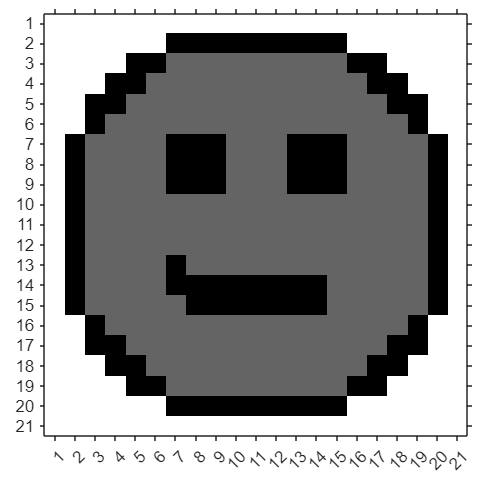
\includegraphics{smiley_mat.png}
    \end{center}
  
    For now, all we'll do is change one of the rows of the image to be all white, and one of the columns to be all black. This can help us see that there's some alignment between matrix notation and how matrices are manipulated in software, and also reinforce the basic idea that matrices are just rows and/or columns of vectors.
  
    First, let's change the $11$th row to be all white. We do this by setting all the values in the $11$th row to $255$. In matrix notation, $11$ is the first index. In MATLAB, we use a colon ``\:'' specify that we want to take all possible columns for the $11$th row.
  
    \begin{verbatim}
    
      smiley(11,:) = 255;
  
    \end{verbatim}
  
    By saying that the $11$th row is equal to $255$, we re-assign the value of each entry to be $255$.
  
    Now let's change the $11$th column to be all black. Using very similar notation, we do the following:
  
    \begin{verbatim}
    
      smiley(:,11) = 0;
  
    \end{verbatim}
  
    Now if we render the figure again, we should see the following:
  
    \begin{center}
      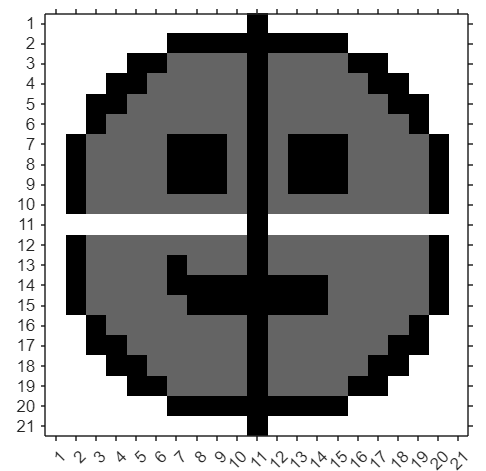
\includegraphics{smiley_mat_changed.png}
    \end{center}
  
    As you can see, the middle row has become white, and the middle column has become black. This is a simple example of how we can manipulate images using matrices.
  
  \end{example}
  
  \end{exploration}

\end{document}